%!TEX program = xelatex

% \documentclass[notes]{beamer}
% \documentclass[notes=only]{beamer}
\documentclass{beamer}

% Good bibliography
\RequirePackage[backend=biber]{biblatex}
\addbibresource[datatype=bibtex]{biblio.bib}

% Icon Fonts
\RequirePackage{academicons}
\RequirePackage{fontawesome}

% Correct the path when including svg pictures
\RequirePackage{import}

% For nice verbatim
\RequirePackage{minted}

% To resize graphic and table
\RequirePackage{graphics}

% For captions
\RequirePackage{caption}

% For quotes
\RequirePackage{csquotes}

% Arrange theme
\usetheme[
	progressbar=frametitle,
	sectionpage=none,
	numbering=fraction
]{metropolis}

\makeatletter
	\setlength{\metropolis@titleseparator@linewidth}{1pt}
	\setlength{\metropolis@progressonsectionpage@linewidth}{2pt}
	\setlength{\metropolis@progressinheadfoot@linewidth}{2pt}
\makeatother

% Color the progress:
% - SciLifeLabGreen (#7FCB28) for SciLifeLab
% - violet for KI
\definecolor{SciLifeLabGreen}{HTML}{7FCB28}
\setbeamercolor{progress bar}{fg=SciLifeLabGreen,bg=white}

\title{Sarek}
\subtitle{The Review - 2018-06-05}
\titlegraphic{\vspace{1.9cm}
	\hfill
\includegraphics[height=.7cm]{pictures/SciLifeLab-white}%

	\hfill
\includegraphics[height=.7cm]{pictures/NGI-white}%

	\hfill
\includegraphics[height=.7cm]{pictures/Barntumorbanken}%
}

\author{\vspace{-.6cm}
	\faUser\ Maxime U. Garcia\\
	\faTwitter\ \href{https://twitter.com/gau/}{@gau}\\
	\faGithub\ \href{https://github.com/MaxUlysse/}{@MaxUlysse}\\
	\faGlobe\ \href{https://maxulysse.github.io/}{maxulysse.github.io}
	\vfill
}

\date{\vfill}

\begin{document}

{
	\usebackgroundtemplate{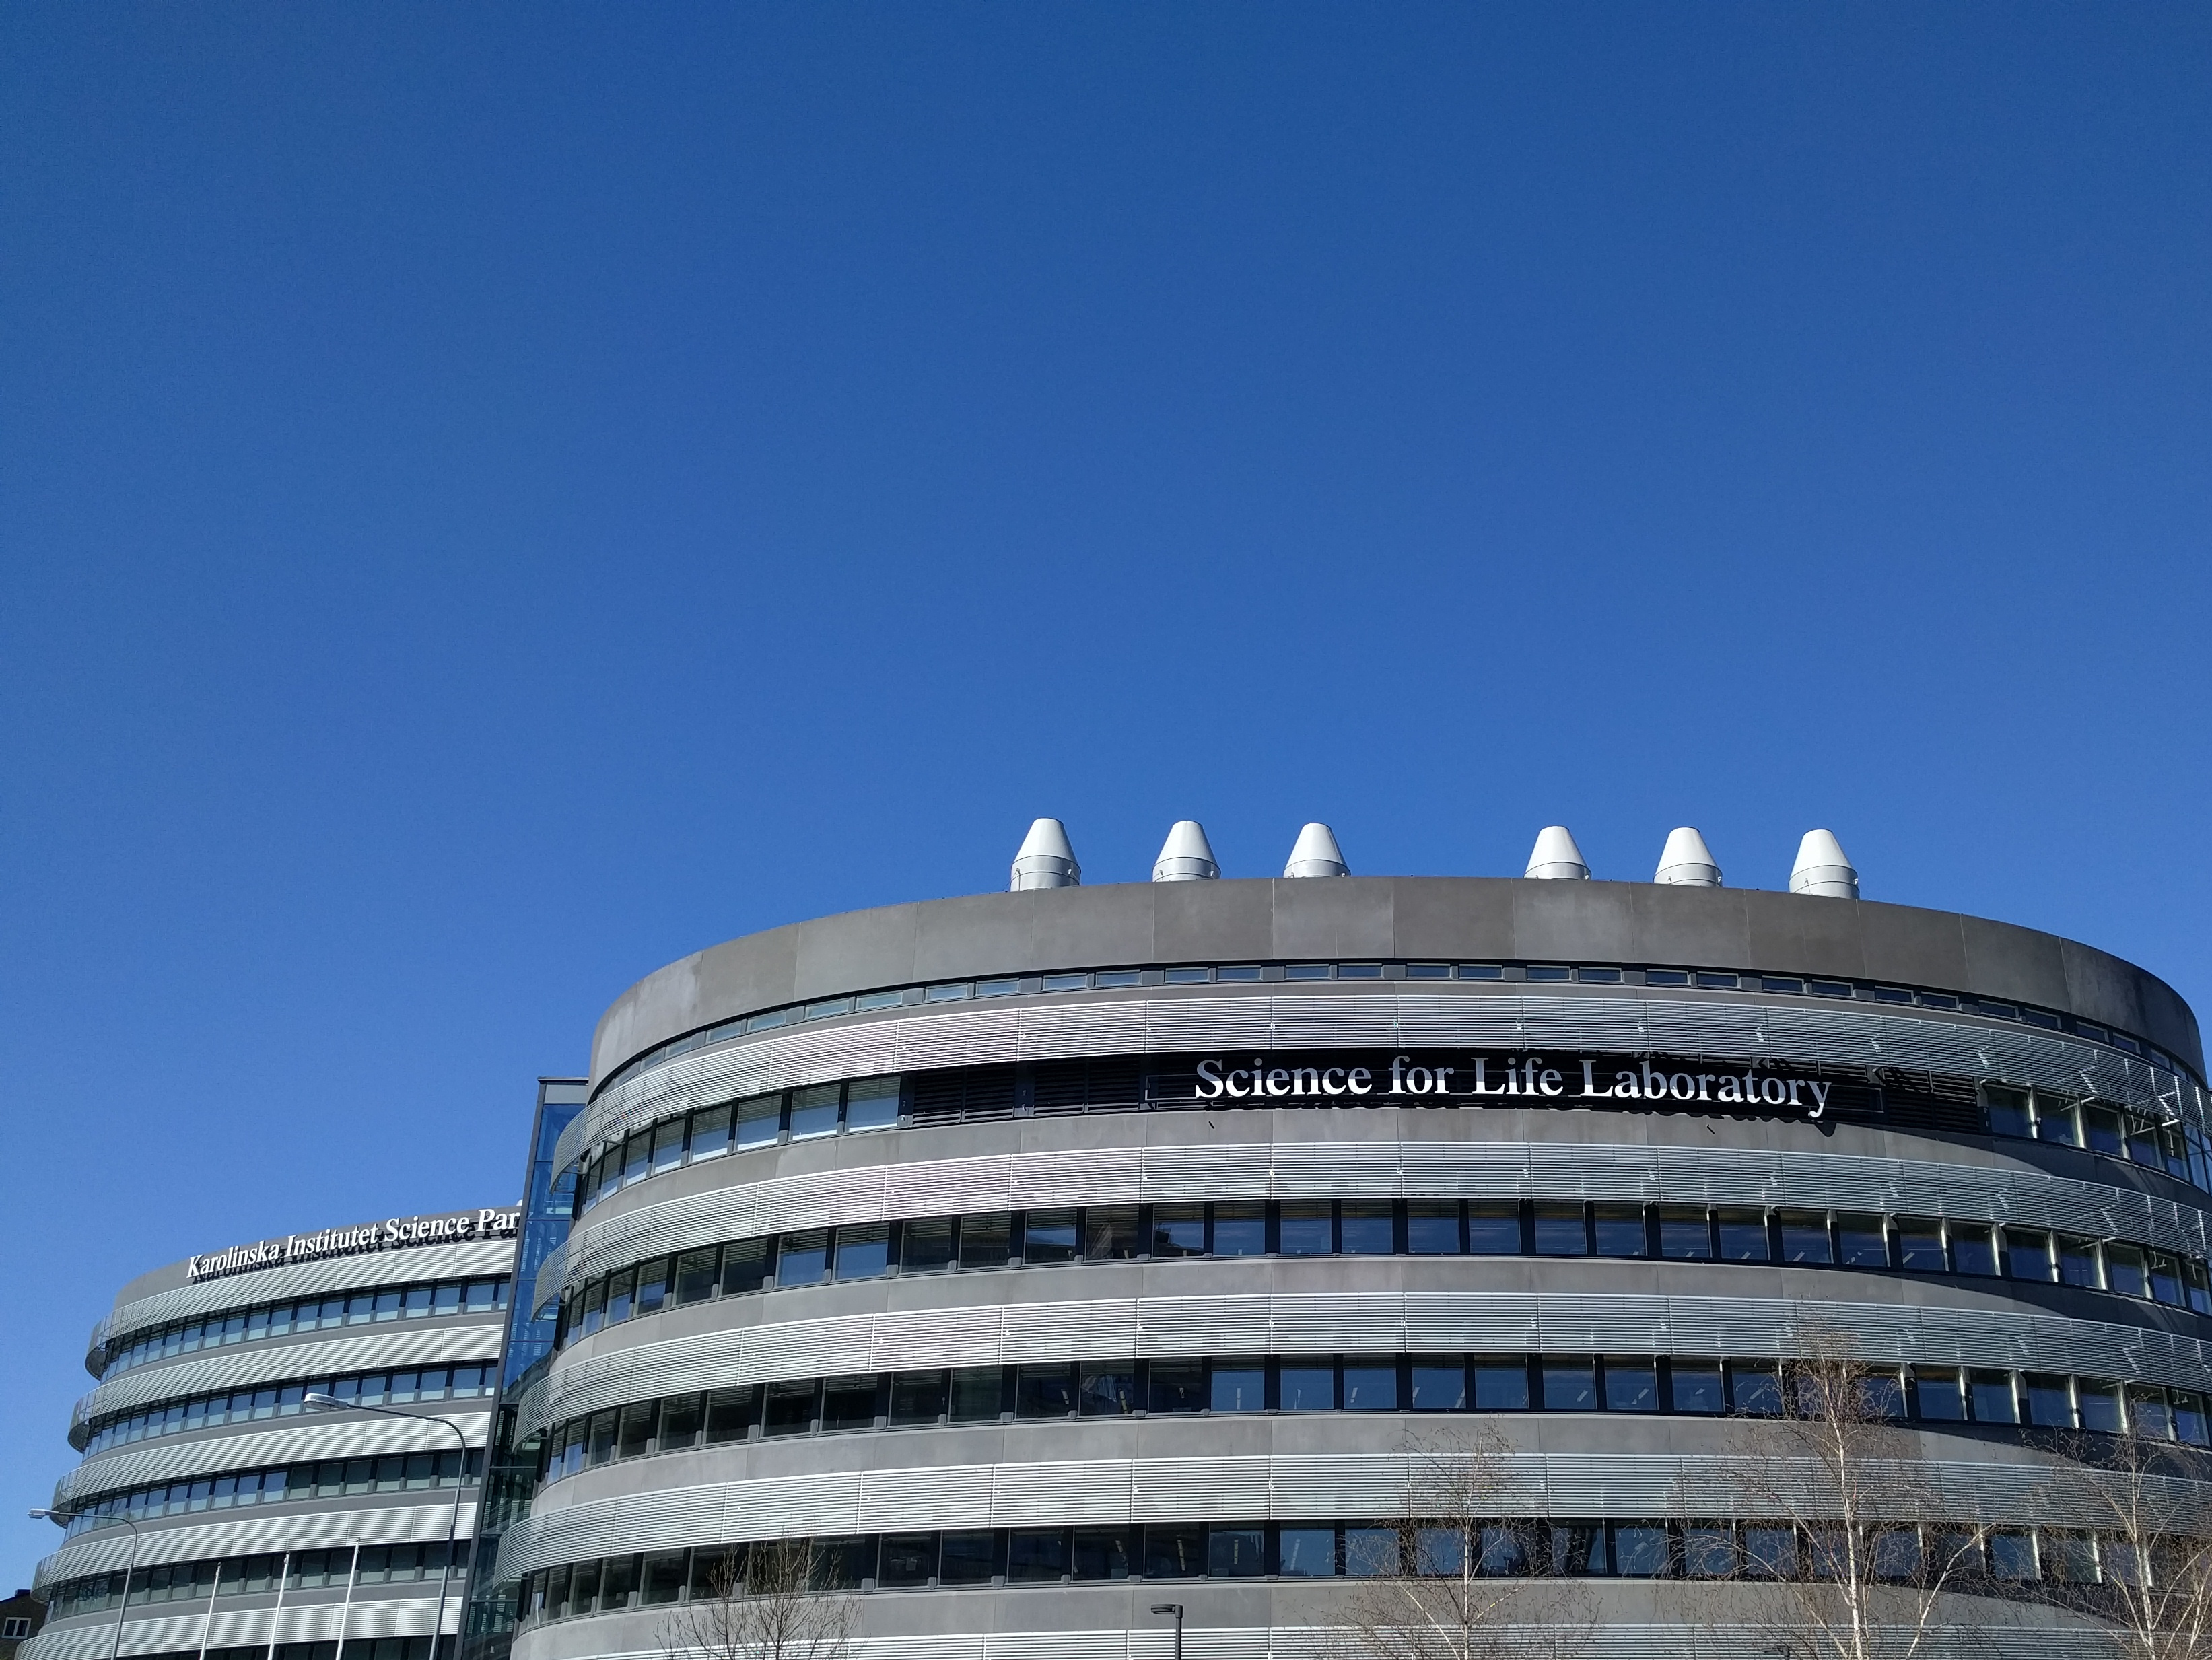
\includegraphics[width=\paperwidth]{pictures/SciLifelab-BlueSky2.jpg}}
	\setbeamercolor{normal text}{fg = white, bg = white}
	\maketitle
}


\section{Agenda}

\begin{frame}{Today's agenda}
	\begin{itemize}
		\item Transition from CAW to Sarek
		\item Article
		\item Deployment on NGI's Irma
		\item Samples with Clinical Genomics
	\end{itemize}
\end{frame}

\section{CAW}

\begin{frame}{Definition}
	\begin{center}
		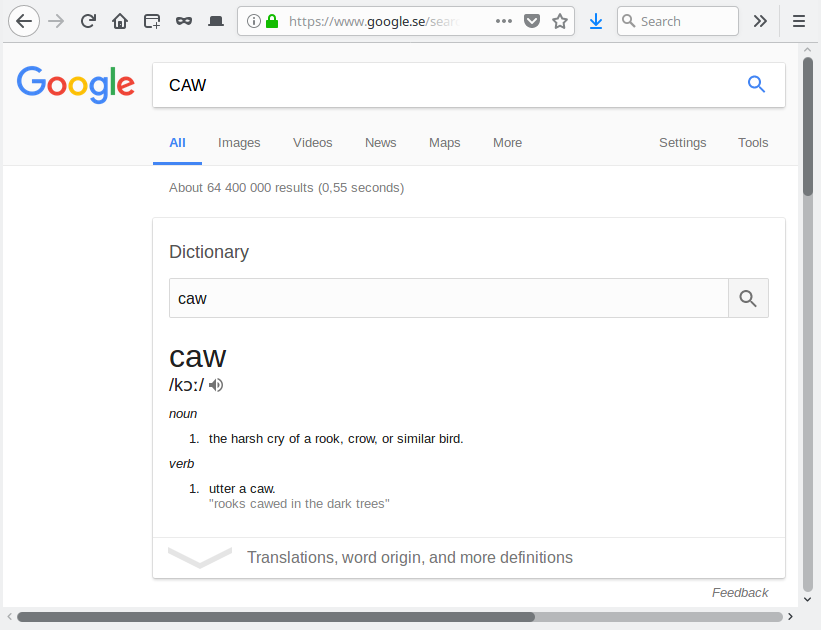
\includegraphics[height=7cm]{pictures/Definition.png}
		\captionof*{figure}{What happens when you look for CAW}
	\end{center}
\end{frame}

\begin{frame}{CAW}
	\begin{center}
		
\includegraphics[height=1cm]{pictures/CAW}
	\end{center}
	\begin{itemize}
		\item Can do more than Tumor/Normal Pair Cancer Analysis
		\pause
		\begin{itemize}
			\item Plan to replace NGI Piper
		\end{itemize}
		\pause
		\item Nobody never really agreed on pronunciation
		\pause
		\begin{itemize}
			\item Get a more Nordic name
		\end{itemize}
	\end{itemize}
\end{frame}

\section{Sarek}

\begin{frame}{Sarek, the National Park}
	\begin{figure}[t]
		\includegraphics[height=7cm]{pictures/Skierfe-summer.jpg}
		\captionof*{figure}{Sarek, the National Park in Northen Sweden}
	\end{figure}
\end{frame}

\begin{frame}{The most dramatic and grandiose of all}
		% Mountains higher than 2,000 metres and almost 100 glaciers.
		\textbf{Long, deep, narrow valleys and wild, turbulent waters}. A tortuous delta landscape.
		% A high alpine area where the Sami people have lived from time immemorial.
		\textbf{Completely lacking in comfortable accommodations}. This is where visitors and the wild World Heritage Site meet.

		Sarek is one of Sweden’s \textbf{most inaccessible national parks} for anyone who cannot hike or ski in on their own. \textbf{There are no roads leading up to the national park}.

		\hfill\href{http://www.nationalparksofsweden.se/choose-park---list/sarek-national-park/national-park-fact/}{Sarek National Park website}
\end{frame}

\begin{frame}{Where we're going we don't need roads}
	\begin{figure}
		
\includegraphics[height=6cm]{pictures/OneDoesNotSimply-meme.png}
	\end{figure}
\end{frame}

% \begin{frame}{Sarek, the Vulcan}
% 	\begin{figure}
% 		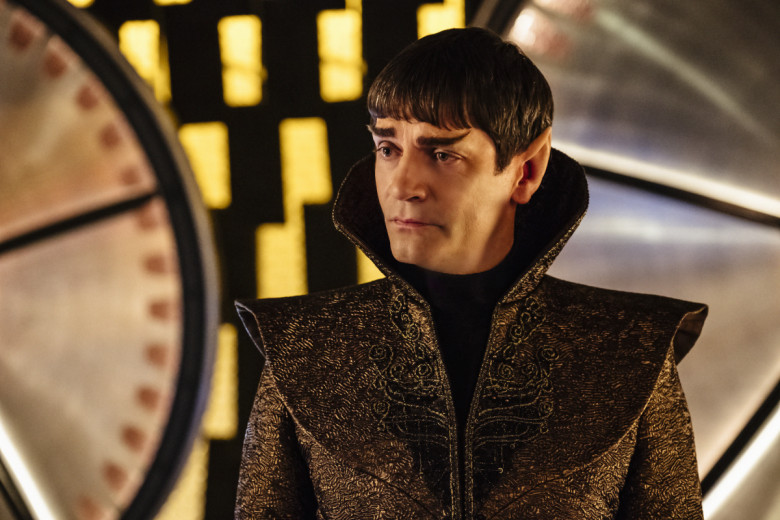
\includegraphics[height=7cm]{pictures/Sarek_discovery.jpg}
% 		\captionof*{figure}{Sarek, portrayed by James Frain in "Star Trek: Discovery"}
% 	\end{figure}
% \end{frame}

\begin{frame}{Quest for a logo}
	\begin{itemize}
		\item More than 50 mails exchanged
	\end{itemize}
	\pause
	\textquote{Any chance you could make the mountain top less pointy? It "hurts" a bit looking at it.}
\end{frame}

\begin{frame}{What is Sarek?}
	\begin{figure}[t]
		
\includegraphics[height=1cm]{pictures/Sarek_no_border}
		\captionof*{figure}{\faGlobe\ \url{http://opensource.scilifelab.se/projects/sarek/}}
	\end{figure}
	\begin{itemize}
		\pause
		\item Nextflow pipeline
		\item<3-> Developed at NGI
		\item<4-> In collaboration with NBIS
		\item<5-> Support from The Swedish Pediatric Tumor Biobank
	\end{itemize}
	\begin{figure}
		
\includegraphics[height=1cm]{pictures/blank}<-2>
		
\includegraphics[height=1cm]{pictures/NGI}<3->
		\only<3->{\hfill}
		
\includegraphics[height=1cm]{pictures/Barntumorbanken}<5->
		\only<4->{\hfill}
		
\includegraphics[height=1cm]{pictures/NBIS}<4->
	\end{figure}
	\vfill
\end{frame}

\begin{frame}{Sarek is now in two flavors}
	\begin{figure}
		
\includegraphics[height=1cm]{pictures/Sarek}
	\end{figure}
	\pause
	\begin{figure}
		
\includegraphics[height=1cm]{pictures/Sarek_germline}
	\end{figure}
	\begin{figure}
		
\includegraphics[height=1cm]{pictures/Sarek_somatic}
	\end{figure}
\end{frame}

\begin{frame}{What does Sarek do?}
	\begin{figure}[t]
		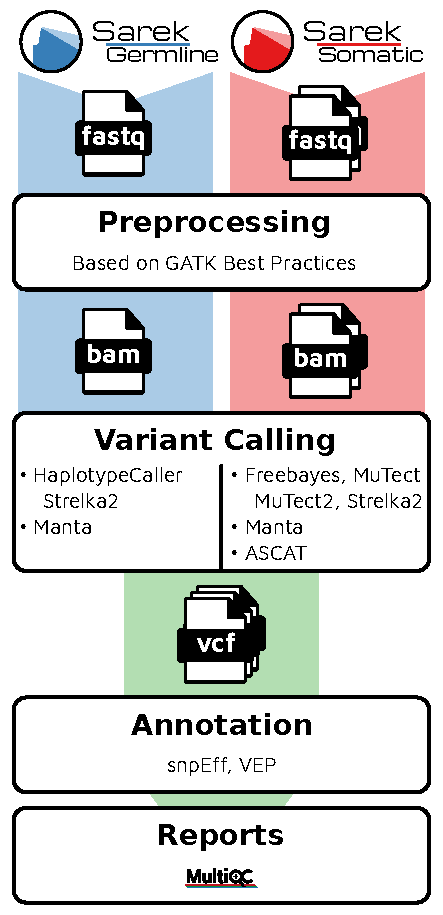
\includegraphics[height=7cm]{pictures/Sarek_workflow_2}
	\end{figure}
\end{frame}

\section{Article}

\begin{frame}{Preprint to BioRxiv and Submission to Bioinformatics}
	\begin{figure}
		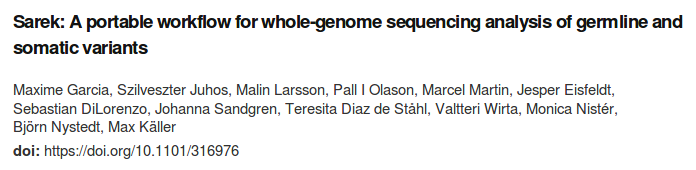
\includegraphics[width=9cm]{pictures/Preprint-Biorxiv.png}
	\end{figure}
	\begin{figure}
		
\includegraphics[width=9cm]{pictures/Manuscript-with-editor.png}
	\end{figure}
\end{frame}

\section{Deployment}

\begin{frame}{Deployed on Irma}
	With the help of:
	\begin{itemize}
		\item Senthil
		\item Pär
	\end{itemize}
	\pause
	Already been used:
	\begin{itemize}
		\item Germline
		\item Somatic
	\end{itemize}
\end{frame}

\section{Clinical Genomics}

\begin{frame}{Collaboration with Clinical Genomics}
\end{frame}

\section{Conferences}

\begin{frame}{Sarek was presented there}
	\begin{itemize}
		\item SPHN Workflow Interoperability Workshop (Basel, Switzerland, 2018/03)
		\item Frontiers in Cancer Research and Therapy (Stockholm, Sweden, 2018/03)
		\item Keystone Symposia - Precision Medicine in Cancer (Stockholm, Sweden, 2018/05)
	\end{itemize}
\end{frame}

\begin{frame}{Sarek will be presented there}
	\begin{itemize}
		\item The Nordic Precision Medicine Initiative (Reykjavik, Iceland, 2018/06)
		\item 25th Biennial Congress Of The European Association For Cancer Research 2018 (Amsterdam, Netherlands, 2018/06-07)
		\item Journées Ouvertes en Biologie, Informatique et Mathématiques (Marseille, France, 2018/07)
	\end{itemize}
\end{frame}

\section{New features}

\begin{frame}{Latest additions}
	\begin{itemize}
		\item New logo and stickers
		\item Main script was dissected into 5 new script
		\begin{itemize}
			\item to facilitate work on separate parts
		\end{itemize}
		\item Follow Strelka Best Practices
		\item Improved slurm usage
		\item Improved help
		\item Improved CI testing
	\end{itemize}
\end{frame}

\section{Discussions}

\begin{frame}{Discussions}
	\begin{itemize}
		\item Control-FREEC
		\item CI testing for ASCAT
		\item GATK 4.0
		\item Removing MuTect1
	\end{itemize}
\end{frame}

\section{Bug reports}

\begin{frame}{Bug reports}
\end{frame}

\section{Acknowledgments}

\begin{frame}{The List of People Involved}
	\begin{figure}
		
\includegraphics[height=1cm]{pictures/Sarek}
	\end{figure}
	\begin{table}
		\resizebox{.8\textwidth}{!}{%
		\begin{tabular}{ll}
			Sebastian DiLorenzo &	Markus Mayrhofer \\
			Jesper Eisfeldt 		&	Monica Nistèr \\
			Phil Ewels					& Björn Nystedt \\
			Maxime Garcia 			&	Pall Olason \\
			Szilveszter Juhos 	&	Markus Ringnér \\
			Max Käller 					&	Pelin Sahlén \\
			Malin Larsson 			&	Johanna Sandgren \\
			Marcel Martin 			&	Teresita Díaz De Ståhl \\
		\end{tabular}}
	\end{table}
\end{frame}

\begin{frame}{Get involved!}
	\begin{itemize}
		\item We are on the SciLifeLab Slack

		\faSlack\ \href{https://scilifelab.slack.com/}{\#sarek-pipeline}
	\end{itemize}
	\pause
	\begin{itemize}
		\item We have a gitter channel

		\faGroup\ \url{https://gitter.im/SciLifeLab/Sarek}
	\end{itemize}
	\pause
	\begin{itemize}
		\item Our code is hosted on Github

		\faGithub\ \url{https://github.com/SciLifeLab/Sarek}
	\end{itemize}
\end{frame}

{
	\usebackgroundtemplate{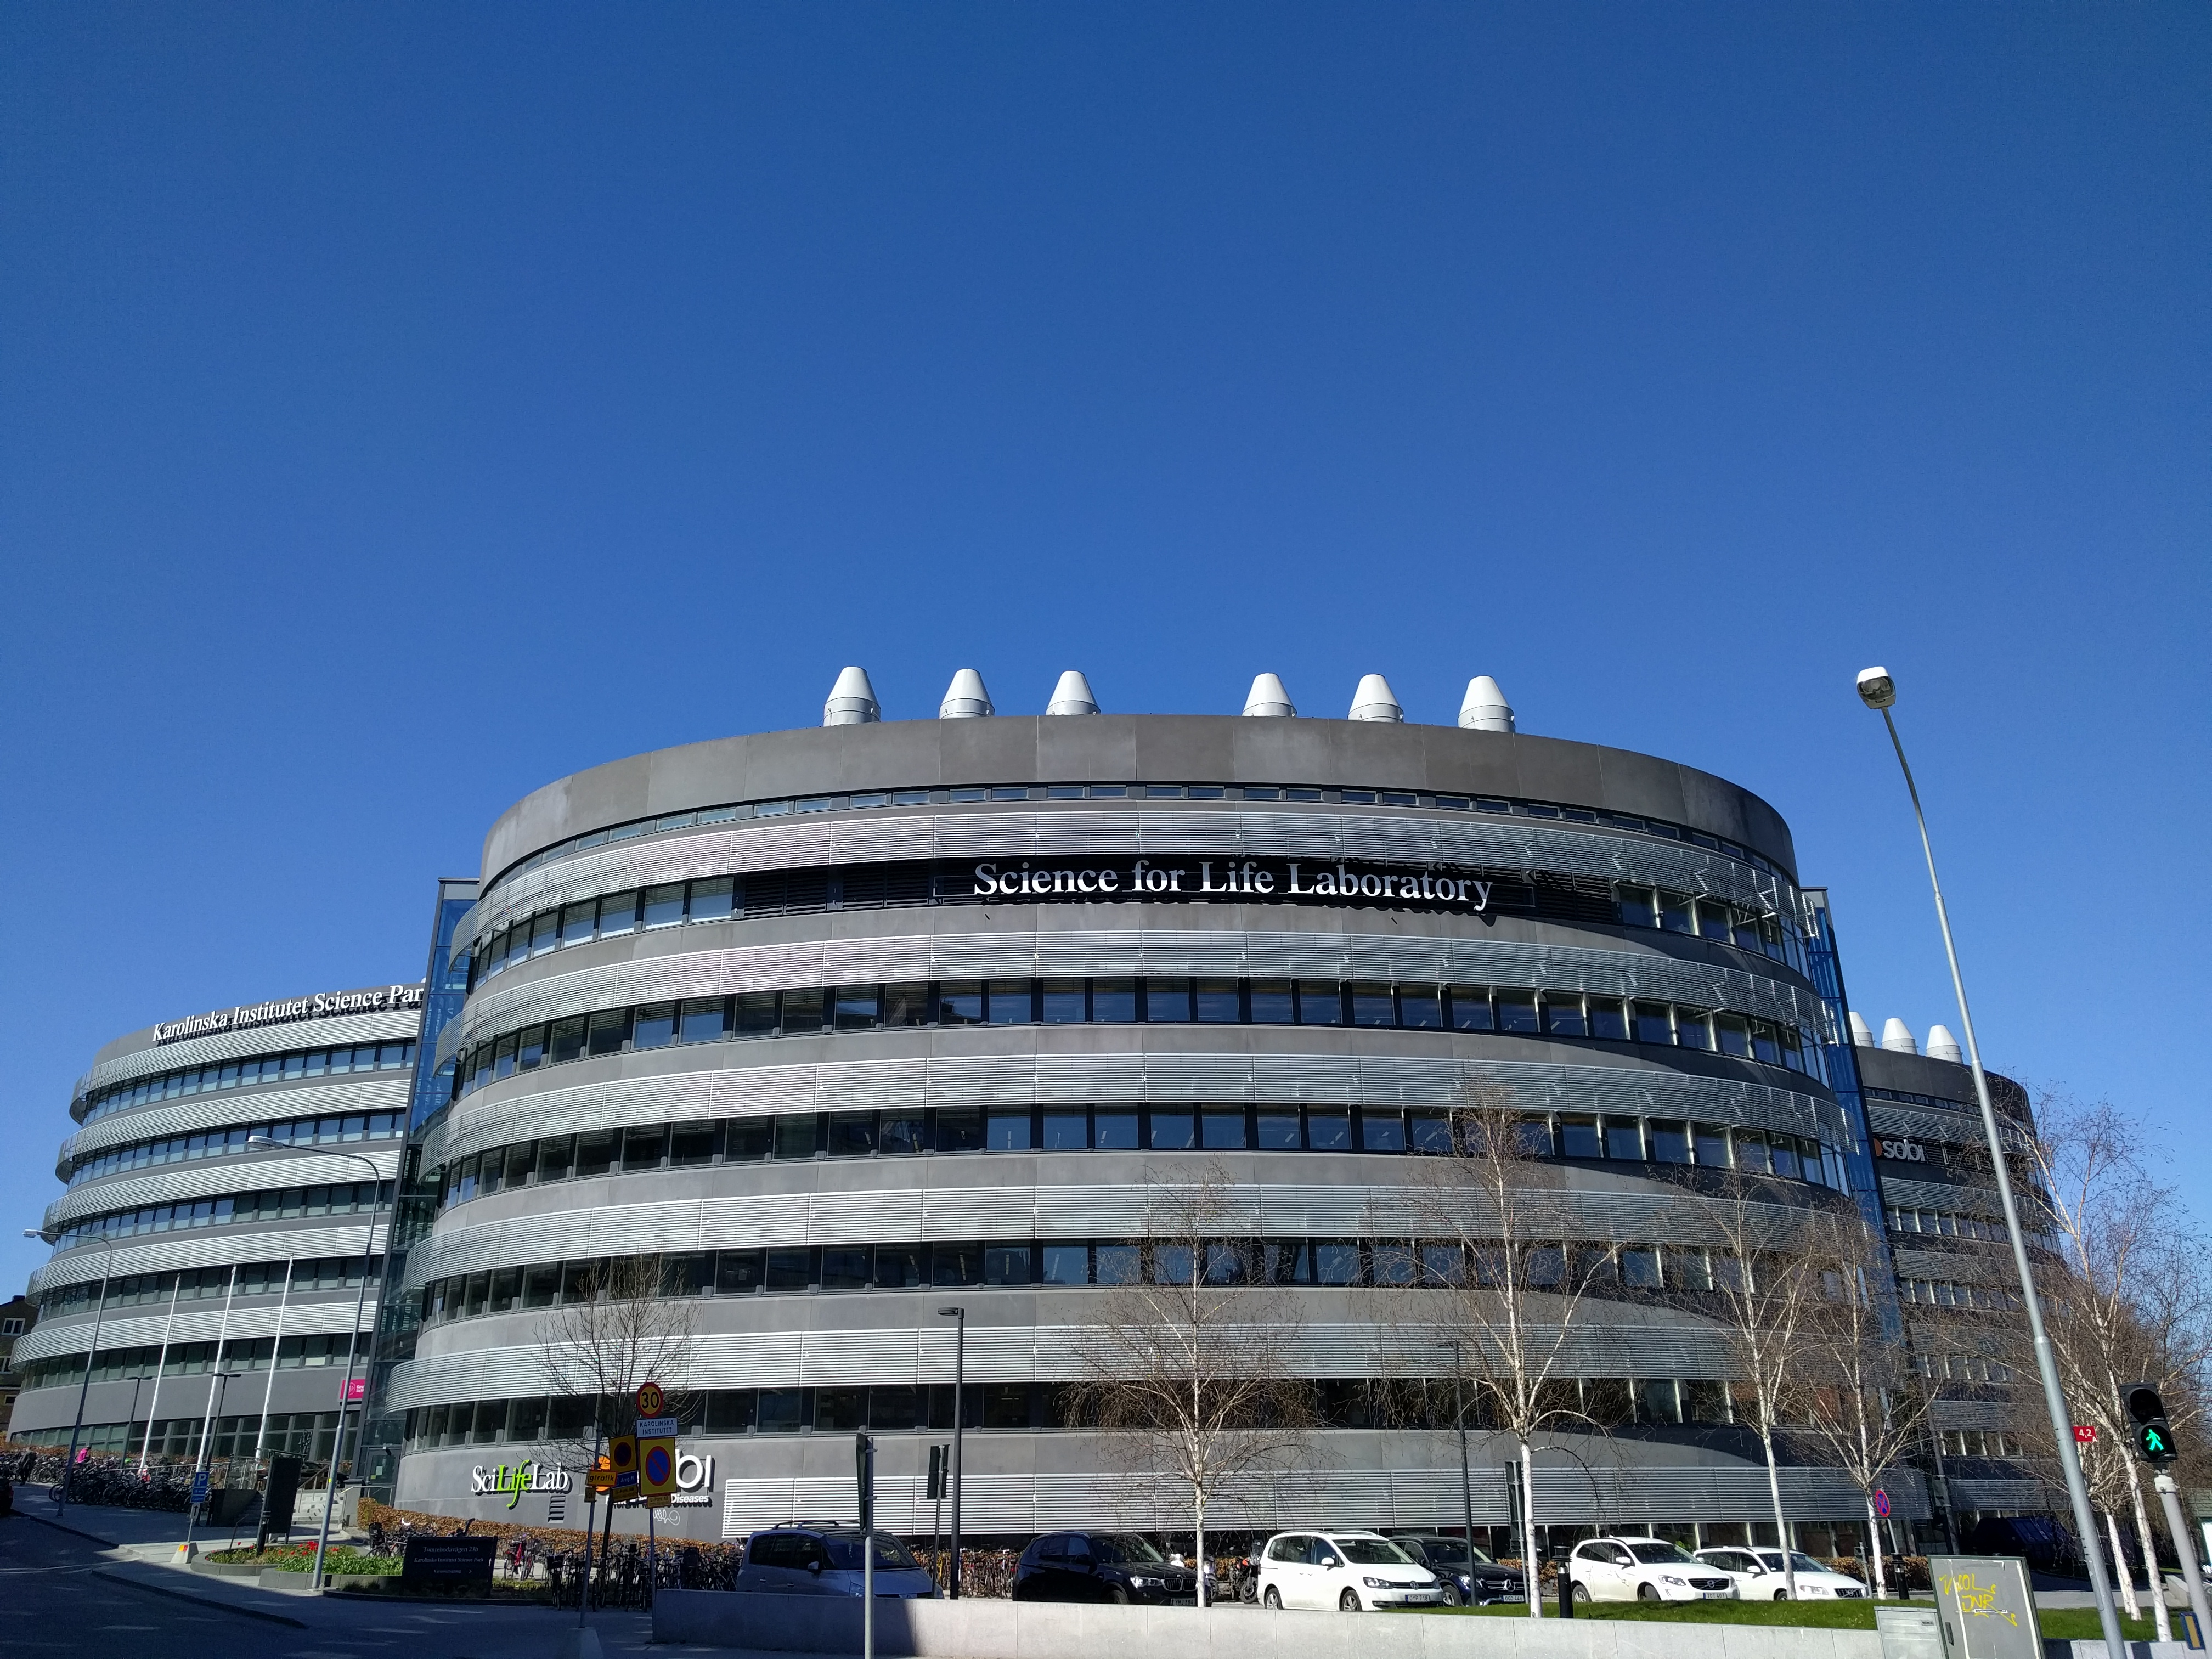
\includegraphics[width=\paperwidth]{pictures/SciLifelab-BlueSky.jpg}}
	\setbeamercolor{normal text}{fg = white}
	\setbeamercolor{frametitle}{fg = white, bg = black!80}
	\usebeamercolor[fg]{normal text}
	\section{Questions}
	\begin{frame}[plain]{Any questions?}
	\vspace{-6cm}
	\faGlobe\ \url{http://opensource.scilifelab.se/projects/sarek/}

	\faGithub\ \url{https://github.com/SciLifeLab/Sarek}
	\end{frame}
}

\end{document}
